\documentclass{article}
\usepackage{tikz}

\begin{document}

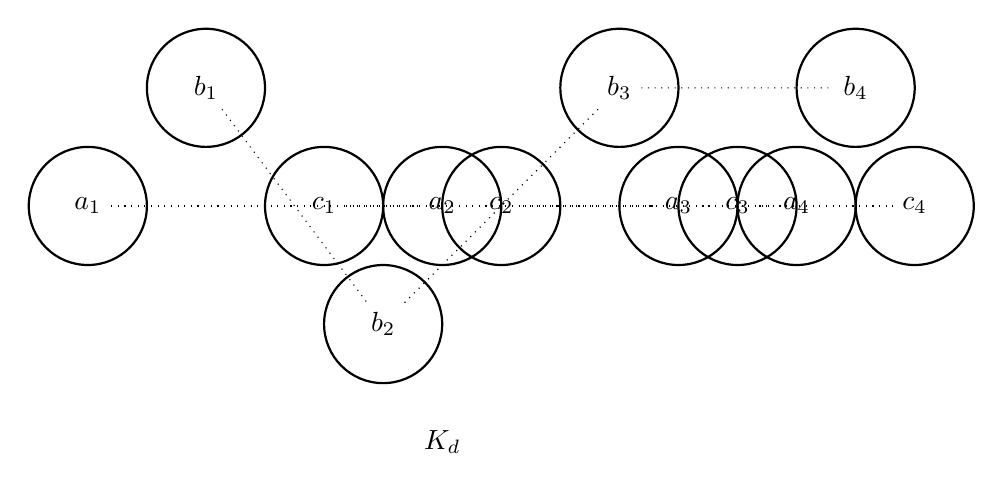
\begin{tikzpicture}[scale=1.5]
    % Define the nodes (centers of circles)
    \node (a1) at (-3, 0) {$a_1$};
    \node (b1) at (-2, 1) {$b_1$};
    \node (c1) at (-1, 0) {$c_1$};
    \node (a2) at (0, 0) {$a_2$};
    \node (b2) at (-0.5, -1) {$b_2$};
    \node (c2) at (0.5, 0) {$c_2$};
    \node (a3) at (2, 0) {$a_3$};
    \node (b3) at (1.5, 1) {$b_3$};
    \node (c3) at (2.5, 0) {$c_3$};
    \node (a4) at (3, 0) {$a_4$};
    \node (b4) at (3.5, 1) {$b_4$};
    \node (c4) at (4, 0) {$c_4$};

    % Draw the circles
    \draw[thick] (a1) circle (0.5);
    \draw[thick] (b1) circle (0.5);
    \draw[thick] (c1) circle (0.5);
    \draw[thick] (a2) circle (0.5);
    \draw[thick] (b2) circle (0.5);
    \draw[thick] (c2) circle (0.5);
    \draw[thick] (a3) circle (0.5);
    \draw[thick] (b3) circle (0.5);
    \draw[thick] (c3) circle (0.5);
    \draw[thick] (a4) circle (0.5);
    \draw[thick] (b4) circle (0.5);
    \draw[thick] (c4) circle (0.5);

    % Draw the dotted lines connecting the centers to K_d
    \draw[dotted] (a1) -- (a2) -- (a3) -- (a4);
    \draw[dotted] (b1) -- (b2) -- (b3) -- (b4);
    \draw[dotted] (c1) -- (c2) -- (c3) -- (c4);

    % Label K_d
    \node at (0, -2) {$K_d$};
\end{tikzpicture}

\end{document}